\section{Experiment}
%Give artists the task to make a video in a certain scene using some specific features, both in Unity and in Maya. We can then compare their performances, and if the two performances are significantly close, the tool was a success.

%Video and audio recordings. Time spent on tasks. Few questions about usability and experience.

%(Hypotheses - not sure yet?)
A test was carried out to find 

What do we want test.

\begin{enumerate}
\item To find out if the FEELS tea's mental models of the camera system match how the system actually works.
\item Compare other artists from TAW 3rd year using the camera system with the FEELS team.
\end{enumerate}


%Figure \ref{fig:test_overview} shows the criteria for the two testing groups \footnote{This will not be in the final paper; it's just for helping you to understand what we mean.}


%\begin{figure}[htbp]
%\centering
%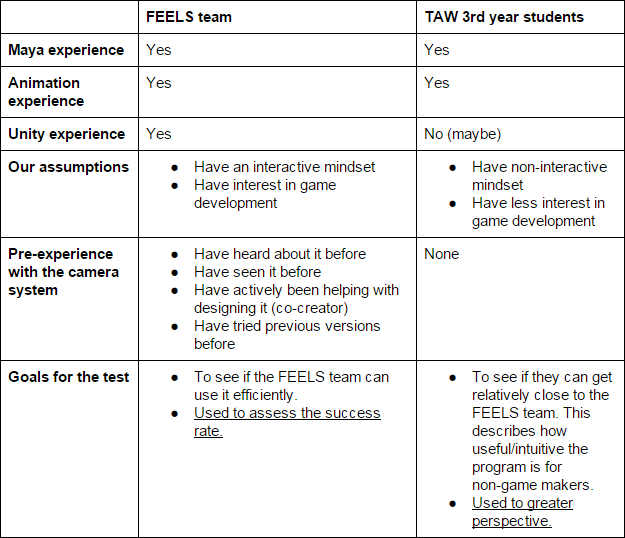
\includegraphics[width=0.5\textwidth]{Pics/test_table_temp}
%\caption{Overview of the testing groups.}
%\label{fig:test_overview}	
%\end{figure}


\subsection{Method} \label{method}

\subsubsection{Participants}
Four male and two female third-year students at The Animation Workshop participated in the test of our camera tool. Three males was from the \textit{Feels} production and one male and the two females was other third-year students no associated with the production. 

\subsubsection{Procedure}
Each participant was tested individually in a small meeting room (see Figure \ref{fig:test_setup}). Besides the participant, a facilitator and an observer was also present in the room. The participant were given a brief introduction and was subsequently presented with a consent form. With their consent, the test began and video recording started. The participants started by answering a demographic questionnaire on a laptop. After this they were introduced to a demo of the Camera Path Animator (see Section \ref{relatedWork}). This was to give the participant context for the test and to introduce them to the concept of camera behaviour in an interactive environment. 

\begin{figure}[htbp]
\centering
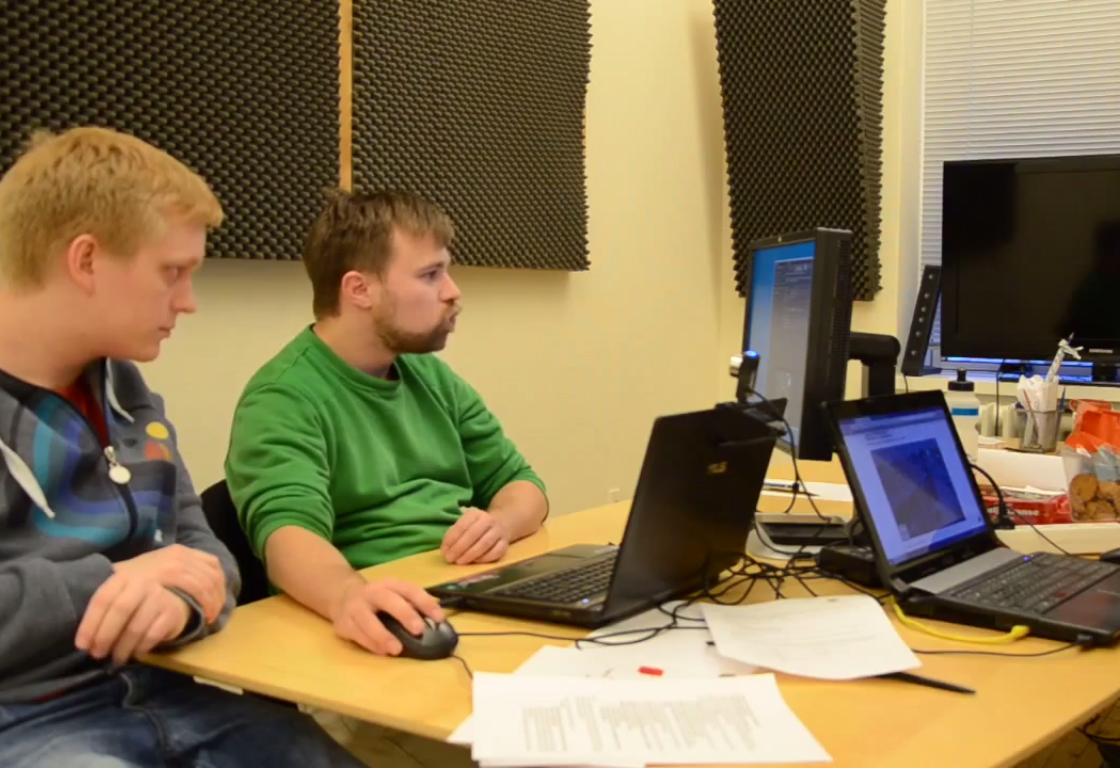
\includegraphics[width=0.3\textwidth]{Pics/test_setup}
\caption{The test participant used had two monitors at his disposal while working with the tool.}
\label{fig:framingConcept}
\end{figure}

The participants and facilitator sat down at another laptop with a second monitor connected. Here the facilitator gave the participant a basic introduction to Unity to ensure that all participants had no problem of navigating and manipulating the workspace. The participant was tasked to move the camera to three specific locations in the environment to ensure they felt comfortable in the workspace. \textbf{Training:} After this the facilitator introduced the camera tool to the participant, first he explained the concept with pen and paper, then he opened the tool in Unity and explained its features and functionalities. The participant was asked to try each feature as they were introduced, e.g. when the facilitator explained how to place influence points and how to connect them, the participant was asked to try it for themselves. \textbf{Tasks:} When all features were explained, and the facilitator felt that the participant had a good grasp on the tool, the participant was handed a piece of paper with 5 tasks such as \textit{"Make the camera's field of view change"} and \textit{"Make the camera go from a low perspective to bird's eye view."} listed on it. The participant had to solve the tasks themselves, the facilitator only intervened when the participant was struggling with something or at unforeseen occurrences (e.g. bugs). \textbf{Creative:} After this, the participant was introduced to a level with a modelled environment. They were then tasked to envision and sketch two ways for the camera to move as the play character moved through this environment, when they had two ideas, they were tasked to implement both of these using our camera tool. The facilitator remained as neutral as possible for this part of the test, but still intervened if they participant was struggling or encountered things like bugs.

Finally, the participant went back to the first laptop and answered a post-test questionnaire. The participant was thanked and the test ended.

\subsubsection{Materials}
Three scenes was constructed for the test. The first was an environment with simple geometry scene. The second was used in the first part of the test when participants were introduced to the camera tool and had to complete 5 tasks. The third level was for the creative part of the test when participants had to envision the camera movement in an environment and then implement it. 

\begin{figure*}[htbp]
\centering
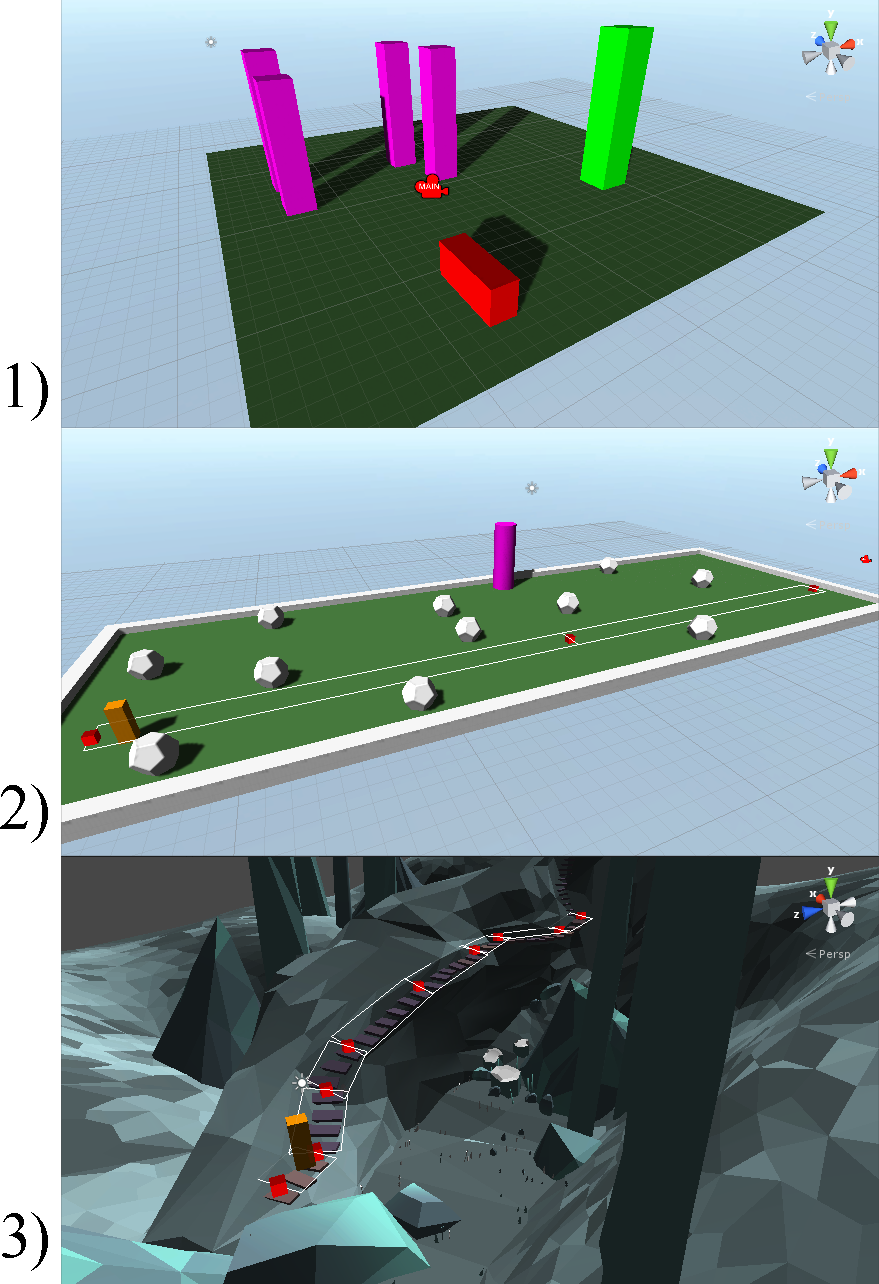
\includegraphics[width=0.45\textwidth]{Pics/sceneAll}
\caption{1) The participant was instructed to move the camera to the top of the green cube, between the purple pillars and to the bottom of the red cube and then rotate the camera to look at the purple pillars. 2) A flat plane with simple geometry to make it easier to see differences when changing camera settings. 3) A mountainous environment with a staircase attached to the mountainside.}
\label{fig:sceneAll}
\end{figure*}

\subsubsection{Data Collection}
The laptop and second monitor was captured using a screen recording software. A webcam feed  that recorded audio and video showing the participant's face was also included in this footage. Additionally, the present observer took notes during the test.

The following are some of the questions which were asked in the post-test questionnaire:

\setlength{\parindent}{1cm}
I felt empowered using this tool

\setlength{\parskip}{0pt}
I felt restricted using this tool

I felt I got the tasks done quick

I felt the tool allowed me to complete the tasks well

\setlength{\parskip}{15pt}
\noindent
Each question's response choice were on a 5-point Likert scale ranging from "strongly disagree" to "strongly agree". Furthermore, they were asked whether they preferred to \textit{'Be the camera'} or taking a \textit{'Snapshot'} for adjusting cameras. They were also asked how useful they thought the instant preview features were. The response choices were "not useful", "somewhat useful", "very useful", "didn't use any of them", and "don't know". To highlight the best features in the tool, the participants were asked to name their favorite feature from a list of 7. To see the full demographic and post-test questionnaire, see APPENDXXACSADSAD. 

\subsubsection{Data Analysis}
how we coded, what we coded for, definitions of terms (success, problem, confusion)...

\subsection{Results} \label{results}
Four participants reported to have between one and three years of experience with Autodesk Maya, another had between four and six years of experience and the last had seven or more years of experience. Only one participant had more than one year of experience with Unity, another had between six and twelve months of experience with it, the rest reported to have less than six months of experience.
When asked if they \textit{'felt empowered using the tool'}, 2/6 participants \textit{strongly agreed} and 4/6 participants \textit{agreed}.

Coded data shows...

When asked if the participants felt empowered using the tool, four participants agreed while the remaining two strongly agreed. When asked if the they felt restricted when using the tool, five participants disagreed while the remaining participant strongly disagreed. To find out how efficient the participants felt using our tool, we asked them if they felt they got the tasks done quick, four participants agreed and two strongly agreed. To find out how effective the participants felt using our tool, we asked them if they felt the tool allowed them to complete the tasks well, three participants agreed and three strongly agreed.
When asked about the preview features, five participants found them very useful, and one found it somewhat useful. For the participants' favorite feature for adjusting camera positions, four named 'Be the camera' and two named 'Snapshot' as their favorite. Furthermore, three participants noted the 'Be the camera' feature as their overall favorite while the 'Slider Preview' was the favorite for the other three participants. 

\subsubsection{Observations}
Quotes, etc...

\subsection{The Three Phases of the Experiment}
\textbf{PHASE 1 - Training:}
\begin{enumerate}
\item Place framings along the movement path so that there's at least one framing in "move path section".
\item Tell the facilitator about the functionality of each button in the interface as you think it'll work.
\item Split a framing connection into two.
\item Delete a framing.
\end{enumerate}

Specific tasks:
\begin{enumerate}
\item Make the camera's field of view change when player gets close to it
\item Make the camera tilt upwards when player gets close to it
\item Make the camera pan to the left when player gets close to it
\item Make the camera look at object X when the player gets close to it
\item Make the camera dolly away from the character as the player walks along a path.
\item Make the camera look from the ground upwards
\item Change the interpolation of one of the previous assignments by changing the animation curve.
\end{enumerate}

\textbf{PHASE 2 - Re-create camera:}
\begin{itemize}
\item Show a video of the end result
\item Recreate this as closely as possible?
\end{itemize}

\textbf{PHASE 3 - Be creative:}
\begin{itemize}
\item Give them environment with path already there, do what you want. Test the limits of the system.
\end{itemize}
